%%%%%%%%%%%%%%%%%%%%%%%%%%%%%%%%%%%%%%%%%%%%%%%%%%%%%%%%%%%%%%%%%%%%%%%%%%%%%%%%
%% Plantilla de memoria en LaTeX para la EIF - Universidad Rey Juan Carlos
%%
%% Por Gregorio Robles <grex arroba gsyc.urjc.es>
%%     Grupo de Sistemas y Comunicaciones
%%     Escuela de Ingeniería de Fuenlabrada
%%     Universidad Rey Juan Carlos
%% (muchas ideas tomadas de Internet, colegas del GSyC, antiguos alumnos...
%%  etc. Muchas gracias a todos)
%%
%% La última versión de esta plantilla está siempre disponible en:
%%     https://github.com/gregoriorobles/plantilla-memoria
%%
%% Para obtener PDF, ejecuta en la shell:
%%   make
%% (las imágenes deben ir en PNG o JPG)

%%%%%%%%%%%%%%%%%%%%%%%%%%%%%%%%%%%%%%%%%%%%%%%%%%%%%%%%%%%%%%%%%%%%%%%%%%%%%%%%

\documentclass[a4paper, 12pt]{book}
%\usepackage[T1]{fontenc}

\usepackage[a4paper, left=2.5cm, right=2.5cm, top=3cm, bottom=3cm]{geometry}
\usepackage{times}
\usepackage[utf8]{inputenc}
\usepackage[spanish]{babel} % Comenta esta línea si tu memoria es en inglés
\usepackage{url}
%\usepackage[dvipdfm]{graphicx}
\usepackage{graphicx}
\usepackage{float}  %% H para posicionar figuras
\usepackage[nottoc, notlot, notlof, notindex]{tocbibind} %% Opciones de índice
\usepackage{latexsym}  %% Logo LaTeX
\usepackage{listings}
% Escribe el título y el nombre del autor / autora para que se use bien
% en otras partes de la plantilla
% Dependiendo de las partes de la plantilla, a veces aparecerán tal
% cual los escribas, a veces totalmente en mayúsculas, a veces de otras
% formas
\title{ANÁLISIS DE AUTORES EN COMÚN DE CONGRESOS Y REVISTAS CIENTÍFICAS USANDO DBLP}
\author{Sergio García Sánchez}

% Guarda el título, el autor y la fecha en variables
\makeatletter
\let\thetitle\@title
\let\theauthor\@author
\let\thedate\@date
\makeatother

\renewcommand{\baselinestretch}{1.5}  %% Interlineado

\begin{document}

\renewcommand{\refname}{Bibliografía}  %% Renombrando
\renewcommand{\appendixname}{Apéndice}


%%%%%%%%%%%%%%%%%%%%%%%%%%%%%%%%%%%%%%%%%%%%%%%%%%%%%%%%%%%%%%%%%%%%%%%%%%%%%%%%
% PORTADA

\begin{titlepage}
\begin{center}
\includegraphics[scale=0.6]{img/URJ_logo_Color_POS.png}

\vspace{1.75cm}

\LARGE
ESCUELA DE INGENIERÍA DE FUENLABRADA
\vspace{1cm}

\LARGE
GRADO EN INGENIERÍA EN SISTEMAS AUDIOVISUALES Y MULTIMEDIA

\vspace{1cm}
\LARGE
\textbf{TRABAJO FIN DE GRADO}

\vspace{2cm}

\Large
\MakeUppercase{\thetitle}

\vspace{2cm}

\large
Autor : \theauthor \\
Tutor : Dr. Gregorio Robles\\
Cotutor: (si procede)
\vspace{1cm}

\large
Curso académico 2023/2024

\end{center}
\end{titlepage}

\newpage
\mbox{}
\thispagestyle{empty} % para que no se numere esta pagina



%%%%%%%%%%%%%%%%%%%%%%%%%%%%%%%%%%%%%%%%%%%%%%%%%%%%%%%%%%%%%%%%%%%%%%%%%%%%%%%%
%%%% Para firmar
\clearpage
\pagenumbering{gobble}
\chapter*{}

\vspace{-4cm}
\begin{center}
\LARGE
\textbf{Trabajo Fin de Grado}

\vspace{1cm}
\large
\thetitle

\vspace{0.8cm}
\large
\textbf{Autor :} \theauthor \\
\textbf{Tutor :} Dr. Nombre del Profesor/a

\end{center}

\vspace{0.8cm}
La defensa del presente Proyecto Fin de Carrera se realizó el día \qquad$\;\,$ de \qquad\qquad\qquad\qquad \newline de 202X, siendo calificada por el siguiente tribunal:


\vspace{0.5cm}
\textbf{Presidente:}

\vspace{1cm}
\textbf{Secretario:}

\vspace{1cm}
\textbf{Vocal:}


\vspace{1cm}
y habiendo obtenido la siguiente \textbf{Calificación:}


\vspace{1cm}
\begin{flushright}
Fuenlabrada, a \qquad$\;\,$ de \qquad\qquad\qquad\qquad de 202X
\end{flushright}

\vspace{1cm}

%% Licencia de publicación en abierto elegida
%% Ver detalles en https://ofilibre.urjc.es/guias/tfg-abierto/
\includegraphics[scale=0.6]{img/by-sa}
%\includegraphics[scale=0.6]{img/by}

%% Poner el año adecuado
\noindent©2024 \theauthor  \\
Algunos derechos reservados  \\
Este documento se distribuye bajo la licencia ``Atribución-CompartirIgual 4.0 Internacional'' de Creative Commons, disponible en \\
\url{https://creativecommons.org/licenses/by-sa/4.0/deed.es}


%%%%%%%%%%%%%%%%%%%%%%%%%%%%%%%%%%%%%%%%%%%%%%%%%%%%%%%%%%%%%%%%%%%%%%%%%%%%%%%%
%%%% Dedicatoria

\chapter*{}
\pagenumbering{Roman} % para comenzar la numeracion de paginas en numeros romanos
\begin{flushright}
\textit{Dedicado a \\
mi familia / mi abuelo / mi abuela}
\end{flushright}

%%%%%%%%%%%%%%%%%%%%%%%%%%%%%%%%%%%%%%%%%%%%%%%%%%%%%%%%%%%%%%%%%%%%%%%%%%%%%%%%
%%%% Agradecimientos

\chapter*{Agradecimientos}
%\addcontentsline{toc}{chapter}{Agradecimientos} % si queremos que aparezca en el índice
\markboth{AGRADECIMIENTOS}{AGRADECIMIENTOS} % encabezado 

Aquí vienen los agradecimientos\ldots Aunque está bien acordarse de la pareja, no hay que olvidarse de dar las gracias a tu madre, que aunque a veces no lo parezca disfrutará tanto de tus logros como tú\ldots 
Además, la pareja quizás no sea para siempre, pero tu madre sí.

%%%%%%%%%%%%%%%%%%%%%%%%%%%%%%%%%%%%%%%%%%%%%%%%%%%%%%%%%%%%%%%%%%%%%%%%%%%%%%%%
%%%% Resumen

\chapter*{Resumen}
%\addcontentsline{toc}{chapter}{Resumen} % si queremos que aparezca en el índice
\markboth{RESUMEN}{RESUMEN} % encabezado

Aquí viene un resumen del proyecto.
Ha de constar de tres o cuatro párrafos, donde se presente de manera clara y concisa de qué va el proyecto. 
Han de quedar respondidas las siguientes preguntas:

\begin{itemize}
  \item ¿De qué va este proyecto? ¿Cuál es su objetivo principal?
  \item ¿Cómo se ha realizado? ¿Qué tecnologías están involucradas?
  \item ¿En qué contexto se ha realizado el proyecto? ¿Es un proyecto dentro de un marco general?
\end{itemize}

Lo mejor es escribir el resumen al final.

%%%%%%%%%%%%%%%%%%%%%%%%%%%%%%%%%%%%%%%%%%%%%%%%%%%%%%%%%%%%%%%%%%%%%%%%%%%%%%%%
%%%% Resumen en inglés

\chapter*{Summary}
%\addcontentsline{toc}{chapter}{Summary} % si queremos que aparezca en el índice
\markboth{SUMMARY}{SUMMARY} % encabezado

Here comes a translation of the ``Resumen'' into English. 
Please, double check it for correct grammar and spelling.
As it is the translation of the ``Resumen'', which is supposed to be written at the end, this as well should be filled out just before submitting.


%%%%%%%%%%%%%%%%%%%%%%%%%%%%%%%%%%%%%%%%%%%%%%%%%%%%%%%%%%%%%%%%%%%%%%%%%%%%%%%%
%%%%%%%%%%%%%%%%%%%%%%%%%%%%%%%%%%%%%%%%%%%%%%%%%%%%%%%%%%%%%%%%%%%%%%%%%%%%%%%%
% ÍNDICES %
%%%%%%%%%%%%%%%%%%%%%%%%%%%%%%%%%%%%%%%%%%%%%%%%%%%%%%%%%%%%%%%%%%%%%%%%%%%%%%%%

% Las buenas noticias es que los índices se generan automáticamente.
% Lo único que tienes que hacer es elegir cuáles quieren que se generen,
% y comentar/descomentar esa instrucción de LaTeX.

%%%% Índice de contenidos
\tableofcontents 
%%%% Índice de figuras
\cleardoublepage
%\addcontentsline{toc}{chapter}{Lista de figuras} % para que aparezca en el indice de contenidos
\listoffigures % indice de figuras
%%%% Índice de tablas
%\cleardoublepage
%\addcontentsline{toc}{chapter}{Lista de tablas} % para que aparezca en el indice de contenidos
%\listoftables % indice de tablas


%%%%%%%%%%%%%%%%%%%%%%%%%%%%%%%%%%%%%%%%%%%%%%%%%%%%%%%%%%%%%%%%%%%%%%%%%%%%%%%%
%%%%%%%%%%%%%%%%%%%%%%%%%%%%%%%%%%%%%%%%%%%%%%%%%%%%%%%%%%%%%%%%%%%%%%%%%%%%%%%%
% INTRODUCCIÓN %
%%%%%%%%%%%%%%%%%%%%%%%%%%%%%%%%%%%%%%%%%%%%%%%%%%%%%%%%%%%%%%%%%%%%%%%%%%%%%%%%

\cleardoublepage
\chapter{Introducción}
\label{sec:intro} % etiqueta para poder referenciar luego en el texto con ~\ref{sec:intro}
\pagenumbering{arabic} % para empezar la numeración de página con números

En este capítulo se introduce el proyecto.
Debería tener información general sobre el mismo, dando la información sobre el contexto en el que se ha desarrollado.

No te olvides de echarle un ojo a la página con los cinco errores de escritura más frecuentes\footnote{\url{http://www.tallerdeescritores.com/errores-de-escritura-frecuentes}}.

Aconsejo a todo el mundo que mire y se inspire en memorias pasadas.
Las memorias de los proyectos que he llevado yo están (casi) todas almacenadas en mi web del GSyC\footnote{\url{https://gsyc.urjc.es/~grex/pfcs/}}.

En mayo de 2023 me apunté a un curso de innovación docente donde nos pidieron hacer un podcast con temática docente. Aproveché entonces para hacer un podcast de unos 30 minutos donde en los primeros quince minutos introducía LaTeX y la memoria, y en los segundos hacía hincapién en aquellas cosas que más os cuestan utilizar en la memoria: las figuras, las tablas y las citas. Podéis escuchar el podcast en Internet\footnote{\url{https://podcasters.spotify.com/pod/show/gregorio-robles9/episodes/Tu-memoria-de-Trabajo-Fin-de-Grado-o-de-Mster-en-LaTeX-e23hucr/a-a58kp2}}.


\section{Sección}
\label{sec:seccion}

Esto es una sección, que es una estructura menor que un capítulo. 

Por cierto, a veces me comentáis que no os compila por las tildes.
Eso es un problema de codificación.
Al guardar el archivo, guardad la codificación de ``ISO-Latin-1'' a ``UTF-8'' (o viceversa) y funcionará.

\subsection{Estilo}
\label{subsec:estilo}

Recomiendo leer los consejos prácticos sobre escribir documentos científicos en \LaTeX \ de Diomidis Spinellis\footnote{\url{https://github.com/dspinellis/latex-advice}}.

Lee sobre el uso de las comas\footnote{\url{http://narrativabreve.com/2015/02/opiniones-de-un-corrector-de-estilo-11-recetas-para-escribir-correctamente-la-coma.html}}. 
Las comas en español no se ponen al tuntún.
Y nunca, nunca entre el sujeto y el predicado (p.ej. en ``Yo, hago el TFG'' sobre la coma).
La coma no debe separar el sujeto del predicado en una oración, pues se cortaría la secuencia natural del discurso.
No se considera apropiado el uso de la llamada coma respiratoria o \emph{coma criminal}.
Solamente se suele escribir una coma para marcar el lugar que queda cuando omitimos el verbo de una oración, pero es un caso que se da de manera muy infrecuente al escribir un texto científico (p.ej. ``El Real Madrid, campeón de Europa'').

A continuación, viene una figura, la Figura~\ref{figura:foro_hilos}. 
Observarás que el texto dentro de la referencia es el identificador de la figura (que se corresponden con el ``label'' dentro de la misma). 
También habrás tomado nota de cómo se ponen las ``comillas dobles'' para que se muestren correctamente. 
Nota que hay unas comillas de inicio (``) y otras de cierre (''), y que son diferentes.
Volviendo a las referencias, nota que al compilar, la primera vez se crea un diccionario con las referencias, y en la segunda compilación se ``rellenan'' estas referencias. 
Por eso hay que compilar dos veces tu memoria.
Si no, no se crearán las referencias.



 \begin{figure}
    \centering
    \includegraphics[bb=0 0 800 600, width=12cm, keepaspectratio]{img/foro1}
    \caption{Página con enlaces a hilos}
    \label{figura:foro_hilos}
 \end{figure}


A continuación un bloque ``verbatim'', que se utiliza para mostrar texto tal cual.
Se puede utilizar para ofrecer el contenido de correos electrónicos, código, entre otras cosas.


{\footnotesize
\begin{verbatim}
    From gaurav at gold-solutions.co.uk  Fri Jan 14 14:51:11 2005
    From: gaurav at gold-solutions.co.uk (gaurav_gold)
    Date: Fri Jan 14 19:25:51 2005
    Subject: [Mailman-Users] mailman issues
    Message-ID: <003c01c4fa40$1d99b4c0$94592252@gaurav7klgnyif>

    Dear Sir/Madam,
    How can people reply to the mailing list?  How do i turn off
    this feature? How can i also enable a feature where if someone
    replies the newsletter the email gets deleted?
    Thanks

    From msapiro at value.net  Fri Jan 14 19:48:51 2005
    From: msapiro at value.net (Mark Sapiro)
    Date: Fri Jan 14 19:49:04 2005
    Subject: [Mailman-Users] mailman issues
    In-Reply-To: <003c01c4fa40$1d99b4c0$94592252@gaurav7klgnyif>
    Message-ID: <PC173020050114104851057801b04d55@msapiro>

    gaurav_gold wrote:
    >How can people reply to the mailing list?  How do i turn off
    this feature? How can i also enable a feature where if someone
    replies the newsletter the email gets deleted?

    See the FAQ
    >Mailman FAQ: http://www.python.org/cgi-bin/faqw-mm.py
    article 3.11
\end{verbatim}
}



\section{Estructura de la memoria}
\label{sec:estructura}


\begin{figure}
  \centering
  \includegraphics[width=9cm, keepaspectratio]{img/arquitectura.png}
  \caption{Estructura del parser básico}
  \label{fig:arquitectura}
\end{figure}




En esta sección se debería introducir la estructura de la memoria. 

Así:


\begin{itemize}
  \item En el primer capítulo se hace una intro al proyecto.
  
  \item En el capítulo~\ref{chap:objetivos} (ojo, otra referencia automática) se muestran los objetivos del proyecto.
  
  \item A continuación se presenta el estado del arte en el capítulo~\ref{chap:estado}.
  
  \item \ldots
\end{itemize}





%%%%%%%%%%%%%%%%%%%%%%%%%%%%%%%%%%%%%%%%%%%%%%%%%%%%%%%%%%%%%%%%%%%%%%%%%%%%%%%%
%%%%%%%%%%%%%%%%%%%%%%%%%%%%%%%%%%%%%%%%%%%%%%%%%%%%%%%%%%%%%%%%%%%%%%%%%%%%%%%%
% OBJETIVOS %
%%%%%%%%%%%%%%%%%%%%%%%%%%%%%%%%%%%%%%%%%%%%%%%%%%%%%%%%%%%%%%%%%%%%%%%%%%%%%%%%

\cleardoublepage % empezamos en página impar
\chapter{Objetivos} % título del capítulo (se muestra)
\label{chap:objetivos} % identificador del capítulo (no se muestra, es para poder referenciarlo)

\section{Objetivo general} % título de sección (se muestra)
\label{sec:objetivo-general} % identificador de sección (no se muestra, es para poder referenciarla)


Mi trabajo fin de grado consiste en crear de una herramienta de análisis de autores que comparten congresos y revistas utilizando DBLP.
Se pretende entender graficamente I)la cantidad de colaboraciones, y II) las dinámicas de publicacion de los autores por congreso, todo dentro
del marco de la comunidad científica.



\section{Objetivos específicos}
\label{sec:objetivos-especificos}

Este proyecto tiene como objetivo crear una herramienta de análisis de autores coincidentes utilizando DBLP, sin embargo, 
este concepto es lo suficientemente amplio como para abordarlo de manera general.Por lo tanto, los objetivos específicos detallan
de la siguiente manera:

1. Decidir las metodología, que tecnologías y proceso tendrá el ecosistema.

2. Desarrollo de la herramienta de visualización de datos:
Para ello se debe implementar:

- La herramienta extracción de datos, procesamiento y ordenación de los mismos.

- Una interfaz gráfica de usuario (WEB) que facilite la interacción y visualización de los datos.

3. Comparación de la interfaz gráfica con la herramienta de conteo de autores por congreso.







\section{Planificación temporal}
\label{sec:planificacion-temporal}

A mí me gusta que aquí pongáis una descripción de lo que os ha llevado realizar el trabajo.
Hay gente que añade un diagrama de GANTT.
Lo importante es que quede claro cuánto tiempo llevas (tiempo natural, p.ej., 6 meses) y a qué nivel de esfuerzo (p.ej., principalmente los fines de semana).


%%%%%%%%%%%%%%%%%%%%%%%%%%%%%%%%%%%%%%%%%%%%%%%%%%%%%%%%%%%%%%%%%%%%%%%%%%%%%%%%
%%%%%%%%%%%%%%%%%%%%%%%%%%%%%%%%%%%%%%%%%%%%%%%%%%%%%%%%%%%%%%%%%%%%%%%%%%%%%%%%
% ESTADO DEL ARTE %
%%%%%%%%%%%%%%%%%%%%%%%%%%%%%%%%%%%%%%%%%%%%%%%%%%%%%%%%%%%%%%%%%%%%%%%%%%%%%%%%

\cleardoublepage
\chapter{Estado del arte}
\label{chap:estado}

        En este capítulo se van a introducir las tecnologías utilizadas en este trabajo.

\section{Python} 
\label{sec:seccion1}

Python ha adquirido una relevancia como lenguaje de programación mas utilizado en la comunidad académica y científica debido a que se trata de un lenguaje de alto nivel, cuya característica principal es sencillez, la versatilidad y la gran colección de bibiliotecas especializadas componen el resto de características mas importantes.

Dentro del contexto de este trabajo, la creación de una herramienta de análisis donde se observa como los autores coinciden en los congresos es muy destacado debido a:

Extracción y la posterior manipulación de datos: Bibliotecas como sqlite3, lmxl o json nos ayuda a convertir los datos en una base de datos manejable.

Web Scraping y APIs: En este apartado destacan las librerías como BeautifulSoup (utilizadas en el comienzo del trabajo) y Request utilizadas para obtención de los datos dentro de la web, incluyendo la recolección de la información de los datos bibliográficos como en este caso DBLP.

Visualización de datos: Bibliotecas como plotly o matplotlib se utilizan para la creación de gráficos detallados de los datos de las publicaciones y colaboraciones entre autores. En este caso se desestimó la idea, ya que como se verá a continuación se desarrolló una herramienta web.

Ventajas de utilizar Python en este proyecto:

Amplia comunidad y soporte: facilidad de acceso a recursos y tutorialesy una amplia comunidad de usuarios y desarrolladores activa.

Eficiencia y simplicidad de uso: Con una sintaxis clara y precisa puedes desarrollar una solución eficiente y rápida.

\subsection{SQlite3}

SQLite3 es una librería en Python que proporciona las herramientas para interactuar con la base de datos de SQlite. Dicha base de datos es una bibliteca de C que implementa un motor de bases de datos SQL autónomo, fiable, sin configuración y con todas las funciones de SQL.

La integración con SQL se produce directamente desde python pudiendo utilizar los comandos: 'SELECT', 'INSERT', 'UPDATE', 'DELETE', como otros operadores de las bases de datos.

No precisa de configuración en un servidor independiente, las bases de datos se almacenan en un archivo del sistema de archivos, facilitando el transporte y su uso. Es importante destacar que cada archivo de base de datos es completamente autónomo y contiene los datos y la lógica necesaria para su funcionamiento.

\subsection{Lxlm}

Se trata de una librería de python que tiene como funciones el procesamiento y manipulación de archivos HTML y XML, es una herramienta con mucho potencial que está construida sobre bibliotecas C, concretamente 'libxslt' y 'libxml2'.

Tiene como características principales la facilidad de uso, compatibilidad con HTML5, manipulación de árboles de datos y destacan el rendimiento y velocidad.

En nuestro trabajo se utiliza para realizar el parseo de información hacia la base de datos en formato SQL.

\subsection{Os}

Biblioteca que proporciona una interfaz para interactuar con el sistema operativo base, permitiendo ejecutar comandos propios del sistema operativo de forma portatil. En nuestra herramiente se utiliza para levantar un error del sistema.

\subsection{Argparse}

Se trata de una librería estandar que proporciona las herramientas para definir los argumentos que precisa una interfaz de línea, como deben procesarse y generan la ayuda para los usuarios. Fue incorporado a Python 2.7 como remplazo de optparse

\subsection{Time}

Biblioteca que suministra las funciones para trabajar con el tiempo, pudiéndose implementar funciones como medir el tiempo de ejecución del programa, gestionar marcas de tiempo o incluir retrasos en el código.

En nuestro trabajo se utiliza para medir la cantidad de tiempo que tarda en realizar el parseo del XML de DBLP.

\subsection{Json}

Módulo que proporciona las herramientas necesarias para la manipulación de archivos JSON. En nuestro proyecto se utiliza para crear el JSON que será leido mediante la API.

\section{JSON} 
\label{sec:seccion1}

JavaScript Object Notation se caracteriza por su simplicidad, legibilidad y compatibilidad con multiples lenguajes de programación, incluyendo como en nuestro caso Python.
Este formato tiene como función almacenar información estructurada que se utiliza para la transferencia de datos entre un servicio web y aplicaciones, principalmente.

Originariamente, JSON se utilizaba con la notación basada en objetos de JavaScript, el formato se compone de dos campos diferenciados key y value.
Las Keys contienen una cadena de caracteres entrecomillada y los Values o valores contienen un tipo de dato válido JSON, del mismo modo entrecomillado. Dicho campo puede estar formado por un array, un string, un objeto, un diccionario, un boolean, un número o un tipo nulo.

En este punto se presenta un ejemplo de la estructura tipo de un formato JSON:

\begin{lstlisting}
{
    "Key": {
        "Dict": {
            "option1": "ok",
            "List": [
                "thing1",
                "thing2",
                "thing3"
            ]
        },
        "Dict2": {
            "opcode": "custom",
            "List2": [
                "customA",
                "customB"
            ]
        }
    }
}
\end{lstlisting}

En el contexto del trabajo, que es la de crear una herramienta de análisis, desempeña un papel fundamental en los siguientes aspectos:

Almacenamiento de datos: Permite almacenar información complicada bien organizada, debido a su estructura flexible y jerárquica. En este trabajo cada autor o publicación se puede almacenar o representar como un objeto JSON con atributos como nombre, año, titulo... Facilitando el manejo y haciéndolo mas accesible.

Intercambio de datos: Como se mencionó anteriormente, es utilizado primordialmente para el intercambio entra servicios web y aplicaciones. La funcionalidad de este trabajo es la de ser extraídos mediante una API, simplificando el análisis y el procesamiento.

Sencillez a la hora de manipular los datos: Se convierte en una tarea mas sencilla debido a la combinación con bibliotecas de Python, que facilitan la escritura, lectura y transformación de la información. 

En conclusión, se trata de un formato muy versatil debido a su compatibilidad multilenguaje, pose flexibilidad y extensibilidad, ya que se puede incorporar nueva información conforme sea necesario y se trata de un formato sencillo y claro a la hora de su visualización.


\section{HTML}

Es el lenguaje utilizado para estructurar y crear páginas web y su contenido. HyperText Markup Languaje fue creado en 1991 y ha ido evolucionando conforme a las necesidades de los usuarios y desarrolladores web.

Desde su comienzo han sido varias las versiones que se han desplegado, destacando HTML 2.0, dicha versión estandarizó muchas funcionalidades y etiquetas que eran soportadas por los navegadores de la época. La versión HTML 4.0 en la cual se introdujo las hojas de estilo CSS. Y la más conocida y actual HTML5, que data del 2014, dicha versión se caracteriza por la inclusión de nuevas etiquetas que dan soporte nativo a las fuentes multimedia, mejora de formularios y soporte para APIs avanzadas.

El impacto provocado por esta versión se caracteriza por la transformación de como se interactua con el contenido en linea. A continuación se detalla las tendencias actuales y futuras que dan forma a la web:

\textbf{Mejoras en posicionamiento SEO y accesibilidad:} Con la incorporación de nuevas etiquetas y atributos permiten a los desarrolladores crear webs que tengan mejor posicionamiento y visibilidad en motores de busqueda y tambien ayuda a ser mas accesibles para personas con discapacidades.

\textbf{Interactividad con WebXR:} Esta tendencia ayuda a abrir nuevas soluciones para interactuar y sumergirte en la web, con la API WebXR ayuda a crear experiencias de realidad virtual (VR) y de realidad aumentada (AR).

\textbf{Aplicaciones web progresivas (PWA):} Esta opción es muy popular entre los desarrolladores que buscan crear aplicaciones que puedan ser utilizadas desde cualquier dispositivo que disponga de un navegador.

\textbf{WebAssembly:} es una tecnología que permite ejecutar codigo de bajo nivel como si se ejecutar de manera nativa. Se utiliza por ejemplo para ejecutar juegos, aplicaciones de calculo o software de edición como si de una aplicación nativa se tratara.

\section{CSS3}
Cascading Style Sheets u hojas de estilo en cascada define como se debe visualizar los elementos de HTML. Está diseñado para discretizar el contenido del documento y la forma de visualizarse dichos datos, se pueden aplicar características tales como los colores, fuentes y capas o layouts.

Se le denomina estilos de cascada ya que se aplican las características de forma jerárquica (de arriba a abajo) siguiendo un patrón de herencia.

\section{NODEJS}

Es un entorno de ejecución de JavaScript implementado bajo el motor de Google Chrome V8, revolucionando el desarrollo de aplicación en la parte del servidor, permitiendo a los desarrolladores utilizar JavaScript tanto en Back-end como en Front-end. Es extremadamente escalable y eficiente para aplicaciones web y servidores puesto que su arquitectura está orientada a eventos y por su modelo de entrada/salida no bloqueante.

Las características principales son:

\begin{itemize}
    \item Arquitectura Orientada a Eventos: Utiliza un bucle de eventos para controlar multiple conexiones simultaneas sin necesidad de establecer nuevos hilos de procesamiento.
    \item Modelo de entrada/salida no bloqueante: Realiza operaciones entrada/salida de manera asíncrona, permitiendo no bloquear el hilo principal.
    \item NPM: Es una colección de modulos y bibliotecas que los desarrolladores pueden utilizar.
    \item Compatibilidad con JSON: Implementa la creación y consumo de APIs RESTful.
    \item Servidor HTTP integrado: Facilidad de crear un servidor web sin necesidad de otros entornos mas complejos como Nginx o Apache.
\end{itemize}

%%%%%%%%%%%%%%%%%%%%%%%%%%%%%%%%%%%%%%%%%%%%%%%%%%%%%%%%%%%%%%%%%%%%%%%%%%%%%%%%
%%%%%%%%%%%%%%%%%%%%%%%%%%%%%%%%%%%%%%%%%%%%%%%%%%%%%%%%%%%%%%%%%%%%%%%%%%%%%%%%
% DISEÑO E IMPLEMENTACIÓN %
%%%%%%%%%%%%%%%%%%%%%%%%%%%%%%%%%%%%%%%%%%%%%%%%%%%%%%%%%%%%%%%%%%%%%%%%%%%%%%%%

\cleardoublepage
\chapter{Diseño e implementación}
\label{sec:diseno}

En este capítulo se va a describir la estructura del software desarrollado, como se han utilizado las herramientas descritas en el apartado anterior.

\section{Arquitectura general} 
\label{sec:arquitectura}

\begin{figure}
  \centering
  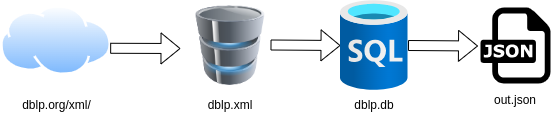
\includegraphics[width=16cm, keepaspectratio]{img/esquemadatos.png}
  \caption{Estructura de transformación de los datos}
  \label{fig:arquitectura}
\end{figure}

Si tu proyecto es un software, siempre es bueno poner la arquitectura (que es cómo se estructura tu programa a ``vista de pájaro'').




Por ejemplo, puedes verlo en la figura~\ref{fig:arquitectura}.
\LaTeX \ pone las figuras donde mejor cuadran. 
Y eso quiere decir que quizás no lo haga donde lo hemos puesto\ldots 
Eso no es malo.
A veces queda un poco raro, pero es la filosofía de \LaTeX: tú al contenido, que yo me encargo de la maquetación.


 
Recuerda que toda figura que añadas a tu memoria debe ser explicada.
Sí, aunque te parezca evidente lo que se ve en la figura~\ref{fig:arquitectura}, la figura en sí solamente es un apoyo a tu texto.
Así que explica lo que se ve en la figura, haciendo referencia a la misma tal y como ves aquí.
Por ejemplo: En la figura~\ref{fig:arquitectura} se puede ver que la estructura del \emph{parser} básico, que consta de seis componentes diferentes: los datos se obtienen de la red, y según el tipo de dato, se pasará a un \emph{parser} específico y bla, bla, bla\ldots

Si utilizas una base de datos, no te olvides de incluir también un diagrama de entidad-relación.


%%%%%%%%%%%%%%%%%%%%%%%%%%%%%%%%%%%%%%%%%%%%%%%%%%%%%%%%%%%%%%%%%%%%%%%%%%%%%%%%
%%%%%%%%%%%%%%%%%%%%%%%%%%%%%%%%%%%%%%%%%%%%%%%%%%%%%%%%%%%%%%%%%%%%%%%%%%%%%%%%
% EXPERIMENTOS Y VALIDACIÓN %
%%%%%%%%%%%%%%%%%%%%%%%%%%%%%%%%%%%%%%%%%%%%%%%%%%%%%%%%%%%%%%%%%%%%%%%%%%%%%%%%

\cleardoublepage
\chapter{Experimentos y validación}
\label{chap:experimentos}

Este capítulo se introdujo como requisito en 2019. 
Describe los experimentos y casos de test que tuviste que implementar para validar tus resultados. 
Incluye también los resultados de validación que permiten afirmar que tus resultados son correctos. 


%%%%%%%%%%%%%%%%%%%%%%%%%%%%%%%%%%%%%%%%%%%%%%%%%%%%%%%%%%%%%%%%%%%%%%%%%%%%%%%%
%%%%%%%%%%%%%%%%%%%%%%%%%%%%%%%%%%%%%%%%%%%%%%%%%%%%%%%%%%%%%%%%%%%%%%%%%%%%%%%%
% RESULTADOS %
%%%%%%%%%%%%%%%%%%%%%%%%%%%%%%%%%%%%%%%%%%%%%%%%%%%%%%%%%%%%%%%%%%%%%%%%%%%%%%%%

\cleardoublepage
\chapter{Resultados}
\label{chap:resultados}

En este capítulo se incluyen los resultados de tu trabajo fin de grado.

Si es una herramienta de análisis lo que has realizado, aquí puedes poner ejemplos de haberla utilizado para que se vea su utilidad.


%%%%%%%%%%%%%%%%%%%%%%%%%%%%%%%%%%%%%%%%%%%%%%%%%%%%%%%%%%%%%%%%%%%%%%%%%%%%%%%%
%%%%%%%%%%%%%%%%%%%%%%%%%%%%%%%%%%%%%%%%%%%%%%%%%%%%%%%%%%%%%%%%%%%%%%%%%%%%%%%%
% CONCLUSIONES %
%%%%%%%%%%%%%%%%%%%%%%%%%%%%%%%%%%%%%%%%%%%%%%%%%%%%%%%%%%%%%%%%%%%%%%%%%%%%%%%%

\cleardoublepage
\chapter{Conclusiones}
\label{chap:conclusiones}


\section{Consecución de objetivos}
\label{sec:consecucion-objetivos}

Esta sección es la sección espejo de las dos primeras del capítulo de objetivos, donde se planteaba el objetivo general y se elaboraban los específicos.

Es aquí donde hay que debatir qué se ha conseguido y qué no. 
Cuando algo no se ha conseguido, se ha de justificar, en términos de qué problemas se han encontrado y qué medidas se han tomado para mitigar esos problemas.

Y si has llegado hasta aquí, siempre es bueno pasarle el corrector ortográfico, que las erratas quedan fatal en la memoria final.
Para eso, en Linux tenemos aspell, que se ejecuta de la siguiente manera desde la línea de \emph{shell}:

\begin{verbatim}
  aspell --lang=es_ES -c memoria.tex
\end{verbatim}

\section{Aplicación de lo aprendido}
\label{sec:aplicacion}

Aquí viene lo que has aprendido durante el Grado/Máster y que has aplicado en el TFG/TFM.
Una buena idea es poner las asignaturas más relacionadas y comentar en un párrafo los conocimientos y habilidades puestos en práctica.

\begin{enumerate}
  \item a
  \item b
\end{enumerate}


\section{Lecciones aprendidas}
\label{sec:lecciones_aprendidas}

Aquí viene lo que has aprendido en el Trabajo Fin de Grado/Máster.

\begin{enumerate}
  \item Aquí viene uno.
  \item Aquí viene otro.
\end{enumerate}


\section{Trabajos futuros}
\label{sec:trabajos_futuros}

Ningún proyecto ni software se termina, así que aquí vienen ideas y funcionalidades que estaría bien tener implementadas en el futuro.

Es un apartado que sirve para dar ideas de cara a futuros TFGs/TFMs.


%%%%%%%%%%%%%%%%%%%%%%%%%%%%%%%%%%%%%%%%%%%%%%%%%%%%%%%%%%%%%%%%%%%%%%%%%%%%%%%%
%%%%%%%%%%%%%%%%%%%%%%%%%%%%%%%%%%%%%%%%%%%%%%%%%%%%%%%%%%%%%%%%%%%%%%%%%%%%%%%%
% APÉNDICE(S) %
%%%%%%%%%%%%%%%%%%%%%%%%%%%%%%%%%%%%%%%%%%%%%%%%%%%%%%%%%%%%%%%%%%%%%%%%%%%%%%%%

\cleardoublepage
\appendix
\chapter{Manual de usuario}
\label{app:manual}

Esto es un apéndice.
Si has creado una aplicación, siempre viene bien tener un manual de usuario.
Pues ponlo aquí.

%%%%%%%%%%%%%%%%%%%%%%%%%%%%%%%%%%%%%%%%%%%%%%%%%%%%%%%%%%%%%%%%%%%%%%%%%%%%%%%%
%%%%%%%%%%%%%%%%%%%%%%%%%%%%%%%%%%%%%%%%%%%%%%%%%%%%%%%%%%%%%%%%%%%%%%%%%%%%%%%%
% BIBLIOGRAFIA %
%%%%%%%%%%%%%%%%%%%%%%%%%%%%%%%%%%%%%%%%%%%%%%%%%%%%%%%%%%%%%%%%%%%%%%%%%%%%%%%%

\cleardoublepage

% Las siguientes dos instrucciones es todo lo que necesitas
% para incluir las citas en la memoria
\bibliographystyle{abbrv}
\bibliography{memoria}  % memoria.bib es el nombre del fichero que contiene
% las referencias bibliográficas. Abre ese fichero y mira el formato que tiene,
% que se conoce como BibTeX. Hay muchos sitios que exportan referencias en
% formato BibTeX. Prueba a buscar en http://scholar.google.com por referencias
% y verás que lo puedes hacer de manera sencilla.
% Más información: 
% http://texblog.org/2014/04/22/using-google-scholar-to-download-bibtex-citations/

\end{document}
